% ---------------------------- README -----------------------------------------
% This file holds section three of the body of the Machine Intelligence II 
% script.
% -----------------------------------------------------------------------------

\setcounter{equation}{0}
\newpage 
\section{Stochastic Optimization}
\label{sec:stochOptimization}
Most supervised and unsupervised learning problems involve
evaluation of a cost function $E^T$. For cost functions with
real-valued arguments, gradient based techniques allow to find
(locally) optimal solutions.

This chapter deals with methods to solve problems based on
cost-functions with \emph{discrete arguments} (e.g.\ cluster
assignment) where gradient-based techniques are not directly
applicable.

% -----------------------------------------------------------------------------

\subsection{Simulated Annealing}
Simulated annealing is a method for stochastic optimization and based on an
{analogy} to ''natural'' optimization. The optimisation algorithm
mimicks freezing or crystallization of a physical system during which
(not necessarily global) optima regarding the energy of the system are reached. The process involves
\emph{slow cooling} (glass vs. crystal $\Rightarrow$ annealing) via
a \emph{computational temperature} $T$ or ''noise parameter'' $\beta =
\frac{1}{T}$.
\\\\
%%%%%%%%%%%%%%%%%%%%%%%%%%%%%%%%%%%%%%%%%%%%%%%%%%%%%%%%%%%%%%%%%%%%%%%%%%%%%%
%% check formatting
%%%%%%%%%%%%%%%%%%%%%%%%%%%%%%%%%%%%%%%%%%%%%%%%%%%%%%%%%%%%%%%%%%%%%%%%%%%%%%
Given a set of \emph{discrete} variables: $\{s_i\}, i = 1, \ldots, N$ (with $s_i \in \mathcal{S}$) describing the \emph{state}\footnote{
we will use short-hand notation: $\vec{s}$ (''state'', but not necessarily a
  vector space)} of the system and a real-valued \emph{cost function}: 
\begin{equation}
	E: \vec{s} \mapsto E_{(\vec{s})} \in \mathbb{R}
\end{equation}
the \emph{goal} is to find the (globally) optimal state $\vec{s}^*$, such that 
\begin{equation}
	E \eqexcl \min 
\end{equation}
``\emph{Stochastic} simulated annealing'' (algorithm \ref{alg:simulatedAnnealing}) implements an iterative procedure to find this optimal state.
\begin{algorithm}[h]
  \DontPrintSemicolon
  initialization: $\vec{s}_0, \tau, M, \beta_0$ small ($\leadsto$ high $T$) \;
  \Begin(Annealing loop: $t=1,2,\dots$){ 
    $\vec{s}_t = \vec{s}_{t-1}$ (initialization of inner loop) \\
    \Begin(State Update loop: $M$ iterations){
      choose a new state $\vec{s}$ randomly (local to $\vec{s}_t$ -- e.g. bit flip)\;
      calculate difference in cost:  $\Delta E = E_{(\vec{s})}
      - E_{(\vec{s}_t)}$ \;
      switch $\vec{s}_t$ to $\vec{s}$ with probability $\mathrm{W}_{(\vec{s}_t \rightarrow \vec{s})} =  
      \frac{1}{1 + \exp( \beta_t \Delta E)}$\;
      (otherwise keep the old state $\vec{s}_t$) \;
      }
      $\beta_t = \tau \beta_{t-1}$  {\tiny (practical but theoretically not optimal)}
    }
    \label{alg:simulatedAnnealing}
    \caption{Stochastic simulated annealing}
  \end{algorithm}
\\
\emph{Remark:} $\vec{s}$ is often chosen ''similar'' or ''close'' to the old state, e.g.\ by randomly ''flipping'' one variable rather than sampling a completely random new state. 
\\\\
The dynamics of such a switching process are affected by the transition probability function $\mathrm{W}$ and its dependence on the temperature parameter $\beta$:
\begin{itemize}
\item transition probability $\mathrm{W}_{(\vec{s}_t \rightarrow \vec{s})}$ 
\begin{figure}[h]
  \centering
    \includegraphics[width=9cm]{section3_fig1}
  \caption{Transition probabilities}
  \label{fig:transition}
\end{figure}
\item limiting cases

\begin{figure}[h] 
  \centering

  \begin{tabular}[h]{c c c}
$T \to \infty, \beta \to 0$ & & $T \to 0, \beta \to \infty$\\
high temperature & & low temperature \\
\begin{tikzpicture}[scale=2.25]
\draw[->] (-1,0) -- (1,0);
\draw[->] (0,0) -- (0,1.25);
\draw[lightgray, very thick] (-1,0.5) -- (.9,0.5);
\draw (0,0) node[anchor=north]{0};
\draw (0,1.25) node[anchor=west]{W};
\draw (1,0) node[anchor=west]{$\Delta E$};
\foreach \y in {0.5,1} \draw (0,\y) node[anchor=south east] {$\y$};
\foreach \y in {0.5,1} \draw (-1pt,\y) -- (1pt,\y);
\end{tikzpicture}
& &
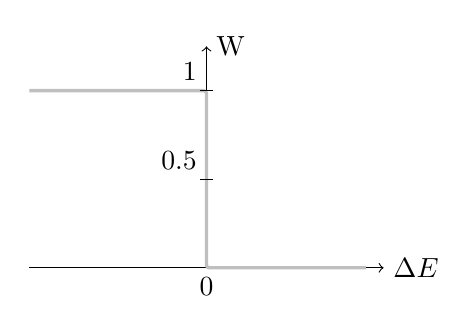
\begin{tikzpicture}[scale=2.25]
\draw[->] (-1,0) -- (1,0);
\draw[->] (0,0) -- (0,1.25);
\draw[lightgray, very thick, rounded corners=1pt](-1,1)-- (0,1) -- (0,0)--(0.9,0);
\draw (0,0) node[anchor=north]{0};
\draw (0,1.25) node[anchor=west]{W};
\draw (1,0) node[anchor=west]{$\Delta E$};
\foreach \y in {0.5,1} \draw (0,\y) node[anchor=south east] {$\y$};
\foreach \y in {0.5,1} \draw (-1pt,\y) -- (1pt,\y);
\end{tikzpicture}
  \end{tabular}
  \caption{Transition probabilities in the two limiting cases}
  \label{fig:transition}
\end{figure}
\end{itemize}
For many optimization problems, the cost function has local optima (see figure \ref{fig:localMinima}). 
\begin{figure}[h]
  \centering
\includegraphics[width=12cm]{section3_fig3}  
  \caption{Cost function with local minima}
  \label{fig:localMinima}
\end{figure}
\begin{figure}[h]
  \centering
\[ \begin{array}{ccc}
	\includegraphics[width=4cm]{section3_fig4}
	& \includegraphics[width=4cm]{section3_fig5}
	& \includegraphics[width=4cm]{section3_fig6} \\\\
	\text{high } T, \text{ low } \beta 
	& \substack{	\text{intermediate values for} \\
			T \text{ and } \beta \\
			\Rightarrow \text{ escape from local} \\
			\text{optima is possible}}
	& \text{low } T, \text{ high } \beta
\end{array} \]
  
  \caption{Effect of annealing on local minima}
\end{figure}
In such cases, convergence to the global optimum of the cost function
is guaranteed if:
\begin{equation}
	\beta_t \sim \ln t
\end{equation}
\begin{itemize}
	\itR robust optimization procedure
	\itR but: $\beta_t \sim \ln t$ is too slow for practical problems
	\itR therefore: $\beta_{t+1} = \tau \beta_t, \tau = 1.01 \ldots 1.30$
		(exponential annealing)
	\itR additionally: the \texttt{State Update loop} has to be iterated often enough, e.g. $M=2000$ ($\leadsto$ thermal equilibrium), 
	however also $M=1$ can work if the temperature is decreased slowly enough
\end{itemize}

% -----------------------------------------------------------------------------

\newpage 						% for visual reasons
\subsection{The Gibbs Distribution}
The random (noisy) state changes cause state fluctuations even for
constant $T$ and $\beta$ (more precisely we have a stochastic process $\vec{s}_{t'}$ with the Markov property). Under certain conditions, these fluctuations
result in a \emph{stationary distribution} over all possible states,
where the probability of observing a specific state depends on its
energy (cost).
\\\\
$\Pi_{(\vec{s}, t')}$: probability distribution across states where $t'$ corresponds to the iteration 
count of the \texttt{State Update loop} of algorithm \ref{alg:simulatedAnnealing}.
\begin{equation}
	\Pi_{(\vec{s}, t')} \rightarrow 
	\underbrace{ P_{(\vec{s})} }_{ \substack{ 	\text{stationary} \\
							\text{distribution}} }
	\text{ for }
	t' \rightarrow \infty \text{ (and constant } T, \beta \text{)}
\end{equation}
calculation of $P_{(\vec{s})}$ under the assumption of "detailed balance" (reversible Markov process): 
\begin{equation}
	\underbrace{ \substack{	\text{probability of} \\
				\text{transition } 
				\vec{s} \rightarrow \vec{s}^{'}} }_{
			P_{(\vec{s})} \mathrm{W}_{(\vec{s} \rightarrow
				\vec{s}^{'})} }
	\underbrace{ = }_{ \substack{	\text{detailed} \\
					\text{balance}}}
	\underbrace{ \substack{	\text{probability of} \\
				\text{transition } 
				\vec{s}^{'} \rightarrow \vec{s} } }_{
			P_{(\vec{s}^{'})} \mathrm{W}_{(\vec{s}^{'} \rightarrow
				\vec{s})} }
\end{equation}
\begin{equation}
	\begin{array}{ll}
	\frac{P_{(\vec{s})}}{P_{(\vec{s}^{'})}}
	& = \frac{\mathrm{W}_{(\vec{s}^{'} \rightarrow \vec{s})}}{
		\mathrm{W}_{(\vec{s} \rightarrow \vec{s}^{'})}} \\\\
	& = \frac{1 + \exp\big\{ \beta \big( E_{(\vec{s})} - E_{(\vec{s}^{'})}
		\big) \big\} }{1 + \exp\big\{ \beta \big( E_{(\vec{s}^{'})} - 
		E_{(\vec{s})}\big) \big\} } \\\\
	& = \frac{1 + \exp( \beta \Delta E)}{1 + \exp( -\beta \Delta E)} \\\\
	& = \exp( \beta \Delta E) \frac{1 + \exp( -\beta \Delta E)}{
		1 + \exp( -\beta \Delta E) } \\\\
	& = \exp( \beta \Delta E )
	\end{array}
\end{equation}
this condition is fulfilled for:
\begin{equation} \tag{Gibbs-Boltzmann-distribution}
	P_{(\vec{s})} = \frac{1}{Z} \exp(-\beta E) 
\end{equation}
normalization constant / partition function (sum over all states):
\begin{equation}
	Z = \sum\limits_{\vec{s}} \exp(-\beta E)
\end{equation}
probability distribution depends on cost and temperature
\begin{figure}[h]
  \centering
\includegraphics[width=12cm]{section3_fig7}  
\[ \begin{array}{ll}
	\beta \downarrow:
	& \text{broad, ''delocalized'' distribution} \\\\
	\beta \uparrow:
	& \text{distribution localized around (global) minima}
\end{array} \]
  \caption{cost-dependent probability distributions}
  \label{fig:costProba}
\end{figure}



% -----------------------------------------------------------------------------

\newpage						% for visual reasons
\subsection{Mean-Field Annealing}
\label{sec:mean-field-annealing}
Stochastic optimization can be computationally expensive: it depends on the cost function $E$ and the cooling schedule.\footnote{so far, we have left $E$ unspecified and -- in many cases -- it will be costly to compute} so a possible strategy might seem to evaluate $P_{(\vec{s})}$ directly ($P_{(\vec{s})}$ is known! -- the Gibbs-distribution). However: 
\begin{itemize}
	\item maxima of $P_{(\vec{s})}$ are equally hard to obtain as minima
		of $E$
	\item moments of $P_{(\vec{s})}$ can - in general - not be calculated
		analytically
\end{itemize}
Fortunately, a viable strategy is to approximate $P_{(\vec{s})}$ by a
computationally tractable distribution $Q_{(\vec{s})}$. 

\paragraph{Approximation:}\label{sec:fact-distr}
The distribution $Q_{(\vec{s})}$ to approximate $P_{(\vec{s})}$ is
chosen as a \emph{factorizing distribution} with costs $E_Q$ linear in
the state variable $\vec{s}$:
\begin{equation}
	Q_{(\vec{s})} \quad
= \quad \frac{1}{Z_Q} \exp \left\{ -\beta E_Q\right\} \quad
= \quad \frac{1}{Z_Q} \exp \Big\{ -\beta \sum\limits_{k}
		\underbrace{ e_k }_{ \text{parameters} } \mathrm{s}_k \Big\}
\end{equation}
\begin{itemize}
	\itr family of distributions parametrized by the \emph{mean fields} $e_k$
      \itr Goal: determine $e_k$ such that this approximation is as good as possible
\end{itemize}

\paragraph{Calculation of moments:}\label{sec:calculation-moments} More generally, moments of a distribution $P$ provide a concise description of $P$. For highly concentrated distributions (e.g.\ $\beta \to \infty$), the
1st moment (its \emph{mean}) gives a good characterization of the distribution
(e.g.\ if it is highly peaked also for the location of its maximum). For the factorizing distribution $Q_{(\vec{s})}$,
these moments can be calculated easily:
\begin{equation}\label{eq:factorizingMoments}
	\Big< f_{(\vec{s}/s_l)} g_{(s_l)} \Big>_Q
	 = \frac{1}{Z_Q} \sum\limits_{\vec{s}} f_{(\vec{s}/s_l)}
		g_{(s_l)} \exp \Big\{ -\beta \sum\limits_k e_k s_k \Big\}
\end{equation}
\begin{eqnarray*}
	& = & \frac{1}{Z_Q} \Bigg[ \sum\limits_{\vec{s}/s_l} f_{(\vec{s}/s_l)}
		\exp \Big( -\beta \sum\limits_{k \neq l} e_k s_k \Big) \Bigg]
		\Bigg[ \sum\limits_{s_l} g_{(s_l)} \exp \Big( -\beta e_l
			s_l \Big) \Bigg] \\\\
	& = & \frac{1}{Z_Q} \Bigg[ \sum\limits_{\vec{s}/s_l} f_{(\vec{s}/s_l)}
		\exp \Big( -\beta \sum\limits_{k \neq l} e_k s_k \Big) \Bigg]
  \frac{\sum\limits_{s_l} \exp(-\beta e_l s_l)}{\sum\limits_{s_l}
		\exp(-\beta e_l s_l)}
		\Bigg[ \sum\limits_{s_l} g_{(s_l)} \exp \Big( -\beta e_l
			s_l \Big) \Bigg] \\\\
	& = &\Big< f_{(\vec{s}/s_l)} \Big>_Q \frac{\sum\limits_{s_l}
		g_{(s_l)} \exp(-\beta e_l s_l)}{\sum\limits_{s_l}
		\exp(-\beta e_l s_l)} \\\\
	& = & \underbrace{ \Big< f_{(\vec{s}/s_l)} \Big>_Q \cdot \Big<g_{(s_l)} 
		\Big>_Q }_{ 	\substack{ \text{factorization of moments} \\
				\rightarrow \text{uncorrelated variables}} }
\end{eqnarray*}
\\
The first moments $\big< s_l \big>_Q$ play a central role in the approximation of $P$ by $Q$ (see below) and usually have a tractable expression:  
% E.g. for $\mathcal{s} = \{0,1\}$  
\begin{equation} \label{eq:mfa_firstmoment_Q}
	\big< s_l \big>_Q = \frac{\sum\limits_{s_l \in \mathcal{S}} s_l \exp(-\beta e_l s_l)}{
					\sum\limits_{s_l \in \mathcal{S}} \exp(-\beta e_l s_l)}
\end{equation}

\paragraph{The mean-field approximation:}
\begin{equation}
	\begin{array}{llc}
	P_{(\vec{s})} 
	& = \frac{1}{Z_p} \exp(-\beta E_p) 
	& \substack{ \text{true distribution} } \\
	Q_{(\vec{s})} 
	& = \frac{1}{Z_Q} \exp\big(-\beta \overbrace{\sum\limits_k e_k s_k}^{E_Q} \big)
	& \substack{ \text{approximation: family of} \\ \text{factorizing distributions} } \\\\
	e_k:
	& \text{\textit{mean fields} }
	& \substack{ \text{parameters to} \\ \text{be determined} }
	\end{array}
\end{equation}
minimization of the KL-divergence:
\begin{equation}
	\dkl(Q||P) = \sum\limits_{\vec{s}} Q_{(\vec{s})} \ln \frac{Q_{(\vec{s})}}{
		P_{(\vec{s})}} \eqexcl \min_{\vec{e}}
\end{equation}
\begin{equation}
	\begin{array}{ll}
	\frac{\partial}{\partial e_l}\dkl
	& = \frac{\partial}{\partial e_l} \bigg\{ \beta \sum\limits_{\vec{s}}
		Q_{(\vec{s})} E_p - \beta \sum\limits_{\vec{s}} 
		Q_{(\vec{s})} E_Q + \ln Z_p - \ln Z_Q \bigg\} \\\\
	& = \beta \frac{\partial}{\partial e_l}\big< E_p \big>_Q
		\underbrace{ -\beta \frac{\partial}{\partial e_l} 
			\sum\limits_{\vec{s}} Q_{(\vec{s})} \sum\limits_k
			e_k s_k }_{ -\beta \sum\limits_k e_k
                        \frac{\partial}{\partial e_l}\big< s_k \big>_Q - \beta
			\big< s_l \big>_Q }
		\underbrace{ -\frac{1}{Z_Q} \sum\limits_{\vec{s}} 
			\frac{\partial}{\partial e_l} \exp(-\beta
			\sum\limits_k e_k s_k) }_{ +\beta \big<s_l\big>_Q }
			\\\\
	& = \beta \frac{\partial}{\partial e_l}\big< E_p \big>_Q -\beta \sum\limits_k 
                        e_k \frac{\partial}{\partial e_l}\big< s_k \big>_Q 
 \qquad \eqexcl \qquad 0
	\end{array}
\end{equation}
The solution to this equation determines the mean fields $e_k$
minimzing $\dkl$ and depends on the exact form of $E_p$. It can be
found by solving the equations:
\begin{equation}\label{eq:MeanfieldEquation}
	\fbox{$ \frac{\partial}{\partial e_l}\big<E_p\big>_Q 
		- \sum\limits_k e_k \frac{\partial}{\partial e_l} \big<s_k\big>_Q = 0
	$}
\end{equation}
The latter simplifies further to 
\begin{equation} \label{eq:mfa_meanfields_simplified}
\fbox{$ \frac{\partial}{\partial e_l}\big<E_p\big>_Q 
		- e_l \frac{\partial}{\partial e_l} \big<s_l\big>_Q = 0
	$}
\end{equation}

because of the independent $\{s_k\}$  under the factorizing distribution $Q$.

\begin{algorithm}[h]
  \DontPrintSemicolon
  initialization: $\langle \vec{s} \rangle_0, \beta_0, t = 0$ \;
  \Begin(Annealing loop){ 
    \Repeat{$|e_k^\mathrm{old}-e_k^\mathrm{new}| < \varepsilon$}
    {
      calculate mean-fields: $e_k, \ \ k = 1, \ldots, N$ \;
      calculate moments: $\big<s_k\big>_Q,\ \ k = 1, \ldots, N$ \;
    }
    increase $\beta$ \;
    }
    \label{alg:MeanFieldAnnealing}
    \caption{Mean Field Annealing}
  \end{algorithm}

\begin{itemize}
	\itR inner loop: fixed-point iteration  for the mean-fields $e_k$
	\itR the moments $\big< s_k \big>$ for not too small temperatures are in general not from the discrete set $\mathcal{S}$ 
	  but range continuously between the elements of $\mathcal{S}$ 
	\itR however: $\beta \rightarrow \infty (T \rightarrow 0): \big< s_k \big>
		\rightarrow s_k^{*}$ \\
		because $P_{(\vec{s})}$ becomes singular at the state 
		$\vec{s}^*$ of minimal cost!
	\itR deterministic (fast) rather than stochastic (slow) optimization
		method (given that mean-field equations can be easily evaluated)
\end{itemize}

see \textcite{BilbroEtAl1989} and \textcite{Rose1998} for details. 
\\

\paragraph{Example (based on Ising model):}
Consider the quadratic cost function $E(s_1, \dots, s_N)$ for binary state vectors, i.e., $s_k \in \mathcal{S} = \{+1, -1\}$,
\begin{equation}
 E_p(\vec{s}) = -\frac{1}{2} \sum\limits_{\substack{i=1,j=1 \\ i\ne j}}^N W_{ij} s_i s_j,
\end{equation}
with a real symmetric matrix $\vec{W}$ with zeros on the diagonal ($\to$ no self-coupling).

The expressions required for the algorithm \ref{alg:MeanFieldAnnealing} can be directly
calculated: 
\begin{enumerate}
 \item The first moment, cf. eq. \eqref{eq:mfa_firstmoment_Q}, become: 
    \begin{align} 
      \big< s_k \big>_Q &= \frac{\sum\limits_{s_k \in \mathcal{S}} s_k \exp(-\beta e_k s_k)}{
					\sum\limits_{s_k \in \mathcal{S}} \exp(-\beta e_k s_k)} \\
			&= \frac{+1 \exp(-\beta e_k) -1 \exp(\beta e_k)}{\exp(-\beta e_k) + \exp(\beta e_k)} \nonumber \\
			&= \tanh(-\beta e_k) \nonumber
    \end{align}
 \item The mean-fields, cf. eq. \eqref{eq:mfa_meanfields_simplified}, are given by 
  \begin{align}
    0 &= \frac{\partial}{\partial e_k}\langle E_p\rangle _Q 
		- e_k \frac{\partial}{\partial e_k} \langle s_k\rangle _Q \\
     &= \frac{\partial}{\partial e_k}\left \langle -\frac{1}{2} 
	  \sum\limits_{\substack{i=1,j=1 \\ i\ne j}}^N W_{ij} s_i s_j \right \rangle_{\substack{Q \\ {} \\ {} \\ {}}} 
		- e_k \frac{\partial}{\partial e_k} \langle s_k\rangle_Q \nonumber \\
     &=  -\frac{1}{2} 
	  \frac{\partial}{\partial e_k} \sum\limits_{\substack{i=1,j=1 \\ i\ne j}}^N W_{ij} \langle s_i \rangle_Q \langle s_j \rangle_Q 
		- e_k \frac{\partial}{\partial e_k} \langle s_k \rangle_Q \nonumber \\
     &= -  \sum\limits_{\substack{i=1 \\ i\ne k}}^N W_{ik} \langle s_i \rangle_Q \frac{\partial}{\partial e_k} \langle s_k \rangle_Q 
		- e_k \frac{\partial}{\partial e_k} \langle s_k\rangle _Q \nonumber
  \end{align}
  which implies
  \begin{equation}
   e_k = -  \sum\limits_{\substack{i=1 \\ i\ne k}}^N W_{ik} \langle s_i \rangle_Q.
  \end{equation}

  Remark: the fixed-point iteration for the mean-fields $\vec{e}$ of this example converges (locally)
  which can be proven
%   \footnote{show: upper bounding the largest eigenvalue of the iteration function's jacobian (having elements
%  with the frobenius norm and show that it remains between $[0,1)$ 
%   i.e., that the iteration 
%   fuction is a contraction} 
using the 
  Banach fixed point theorem (at least for sufficiently large $\beta$).
\end{enumerate}


% -----------------------------------------------------------------------------
